\chapter{Simulazione e Analisi dei Guasti} \label{chap:guasti}

In questo capitolo viene affrontato il Punto 3 del progetto: l'implementazione dei guasti descritti nelle specifiche e la verifica del comportamento del sistema controllato in presenza di tali anomalie. Come richiesto, l'analisi si concentra sulla risposta del controllore nominale (progettato nel Capitolo \ref{chap:tracking}) quando il sistema reale diverge dal modello ideale.

\section{Modellistica dei Guasti}
I guasti sono modellati come variazioni moltiplicative dell'efficienza degli attuatori. Le equazioni cinematiche reali diventano:
\begin{align}
    \dot{\varphi}_1 &= w_1 u_1 \\
    \dot{\varphi}_2 &= w_2 u_2
\end{align}
dove \( w_1, w_2 \in [0, 1] \) sono i parametri di efficienza (1 = nominale, 0 = guasto totale).

Come da Tabella 2 delle specifiche, sono stati considerati i seguenti scenari:
\begin{itemize}
    \item \textbf{FD1 (Rallentamento Ruota DX):} \( w_1 \in (0,1), w_2=1 \).
    \item \textbf{FS1 (Rallentamento Ruota SX):} \( w_1=1, w_2 \in (0,1) \).
    \item \textbf{FD2 (Blocco Ruota DX):} \( w_1=0, w_2=1 \).
    \item \textbf{FS2 (Blocco Ruota SX):} \( w_1=1, w_2=0 \).
\end{itemize}

\section{Setup della Simulazione}
Per valutare l'impatto dei guasti, è stato predisposto un test con le seguenti caratteristiche:
\begin{itemize}
    \item \textbf{Traiettoria:} Circolare (\( R=5 \) m, \( \omega_{ref}=0.3 \) rad/s).
    \item \textbf{Istante di Guasto:} \( T_{fault} = 20 \) s.
    \item \textbf{Scenario Testato:} FD1 con \( w_1 = 0.6 \) (perdita del 40\% di efficienza sulla ruota destra).
    \item \textbf{Controllore:} Nominale (Feedback Linearization), ignaro del guasto.
\end{itemize}

\section{Analisi dei Risultati}
I risultati della simulazione sono riportati in Figura \ref{fig:punto3_results}.

\subsection{Analisi della Traiettoria (Grafico sx)}
Fino all'istante \( t = 20 \) s (segnato con una croce rossa "Inizio Guasto"), il robot segue perfettamente la circonferenza di riferimento (linea nera tratteggiata). 
Appena il guasto si attiva, la ruota destra inizia a girare più lentamente del previsto (\( \dot{\varphi}_1 = 0.6 u_1 \)). Poiché la ruota destra è quella esterna alla curva (il robot gira in senso antiorario), una sua perdita di potenza causa una riduzione del raggio di curvatura istantaneo.
Di conseguenza, il robot "stringe" la curva, deviando verso l'interno e allontanandosi progressivamente dalla traiettoria desiderata (linea blu continua che spiraleggia verso l'interno).

\subsection{Analisi Parametrica ed Errore (Grafici dx)}
\begin{itemize}
    \item \textbf{Parametri di Efficienza (Alto dx):} Il grafico mostra l'evoluzione temporale dei parametri \( w \). Si nota chiaramente il gradino discendente della linea blu (\( w_1 \)) che passa da 1.0 a 0.6 all'istante \( t=20 \) s, mentre \( w_2 \) (linea rossa) rimane costante a 1.0.
    
    \item \textbf{Errore di Posizione (Basso dx):} L'errore lungo gli assi X e Y è nullo nella prima fase. A \( t=20 \) s, gli errori iniziano a crescere rapidamente. L'andamento oscillatorio e divergente degli errori \( e_x \) (rosso) ed \( e_y \) (blu) conferma che il controllore nominale non è in grado di compensare un guasto di questa entità: pur tentando di correggere, il modello inverso utilizzato per il calcolo di \( u \) è ormai errato rispetto alla realtà fisica del veicolo.
\end{itemize}

\begin{figure}[h]
    \centering
    % Assicurati che il file si chiami 'PuntoN3.png'
    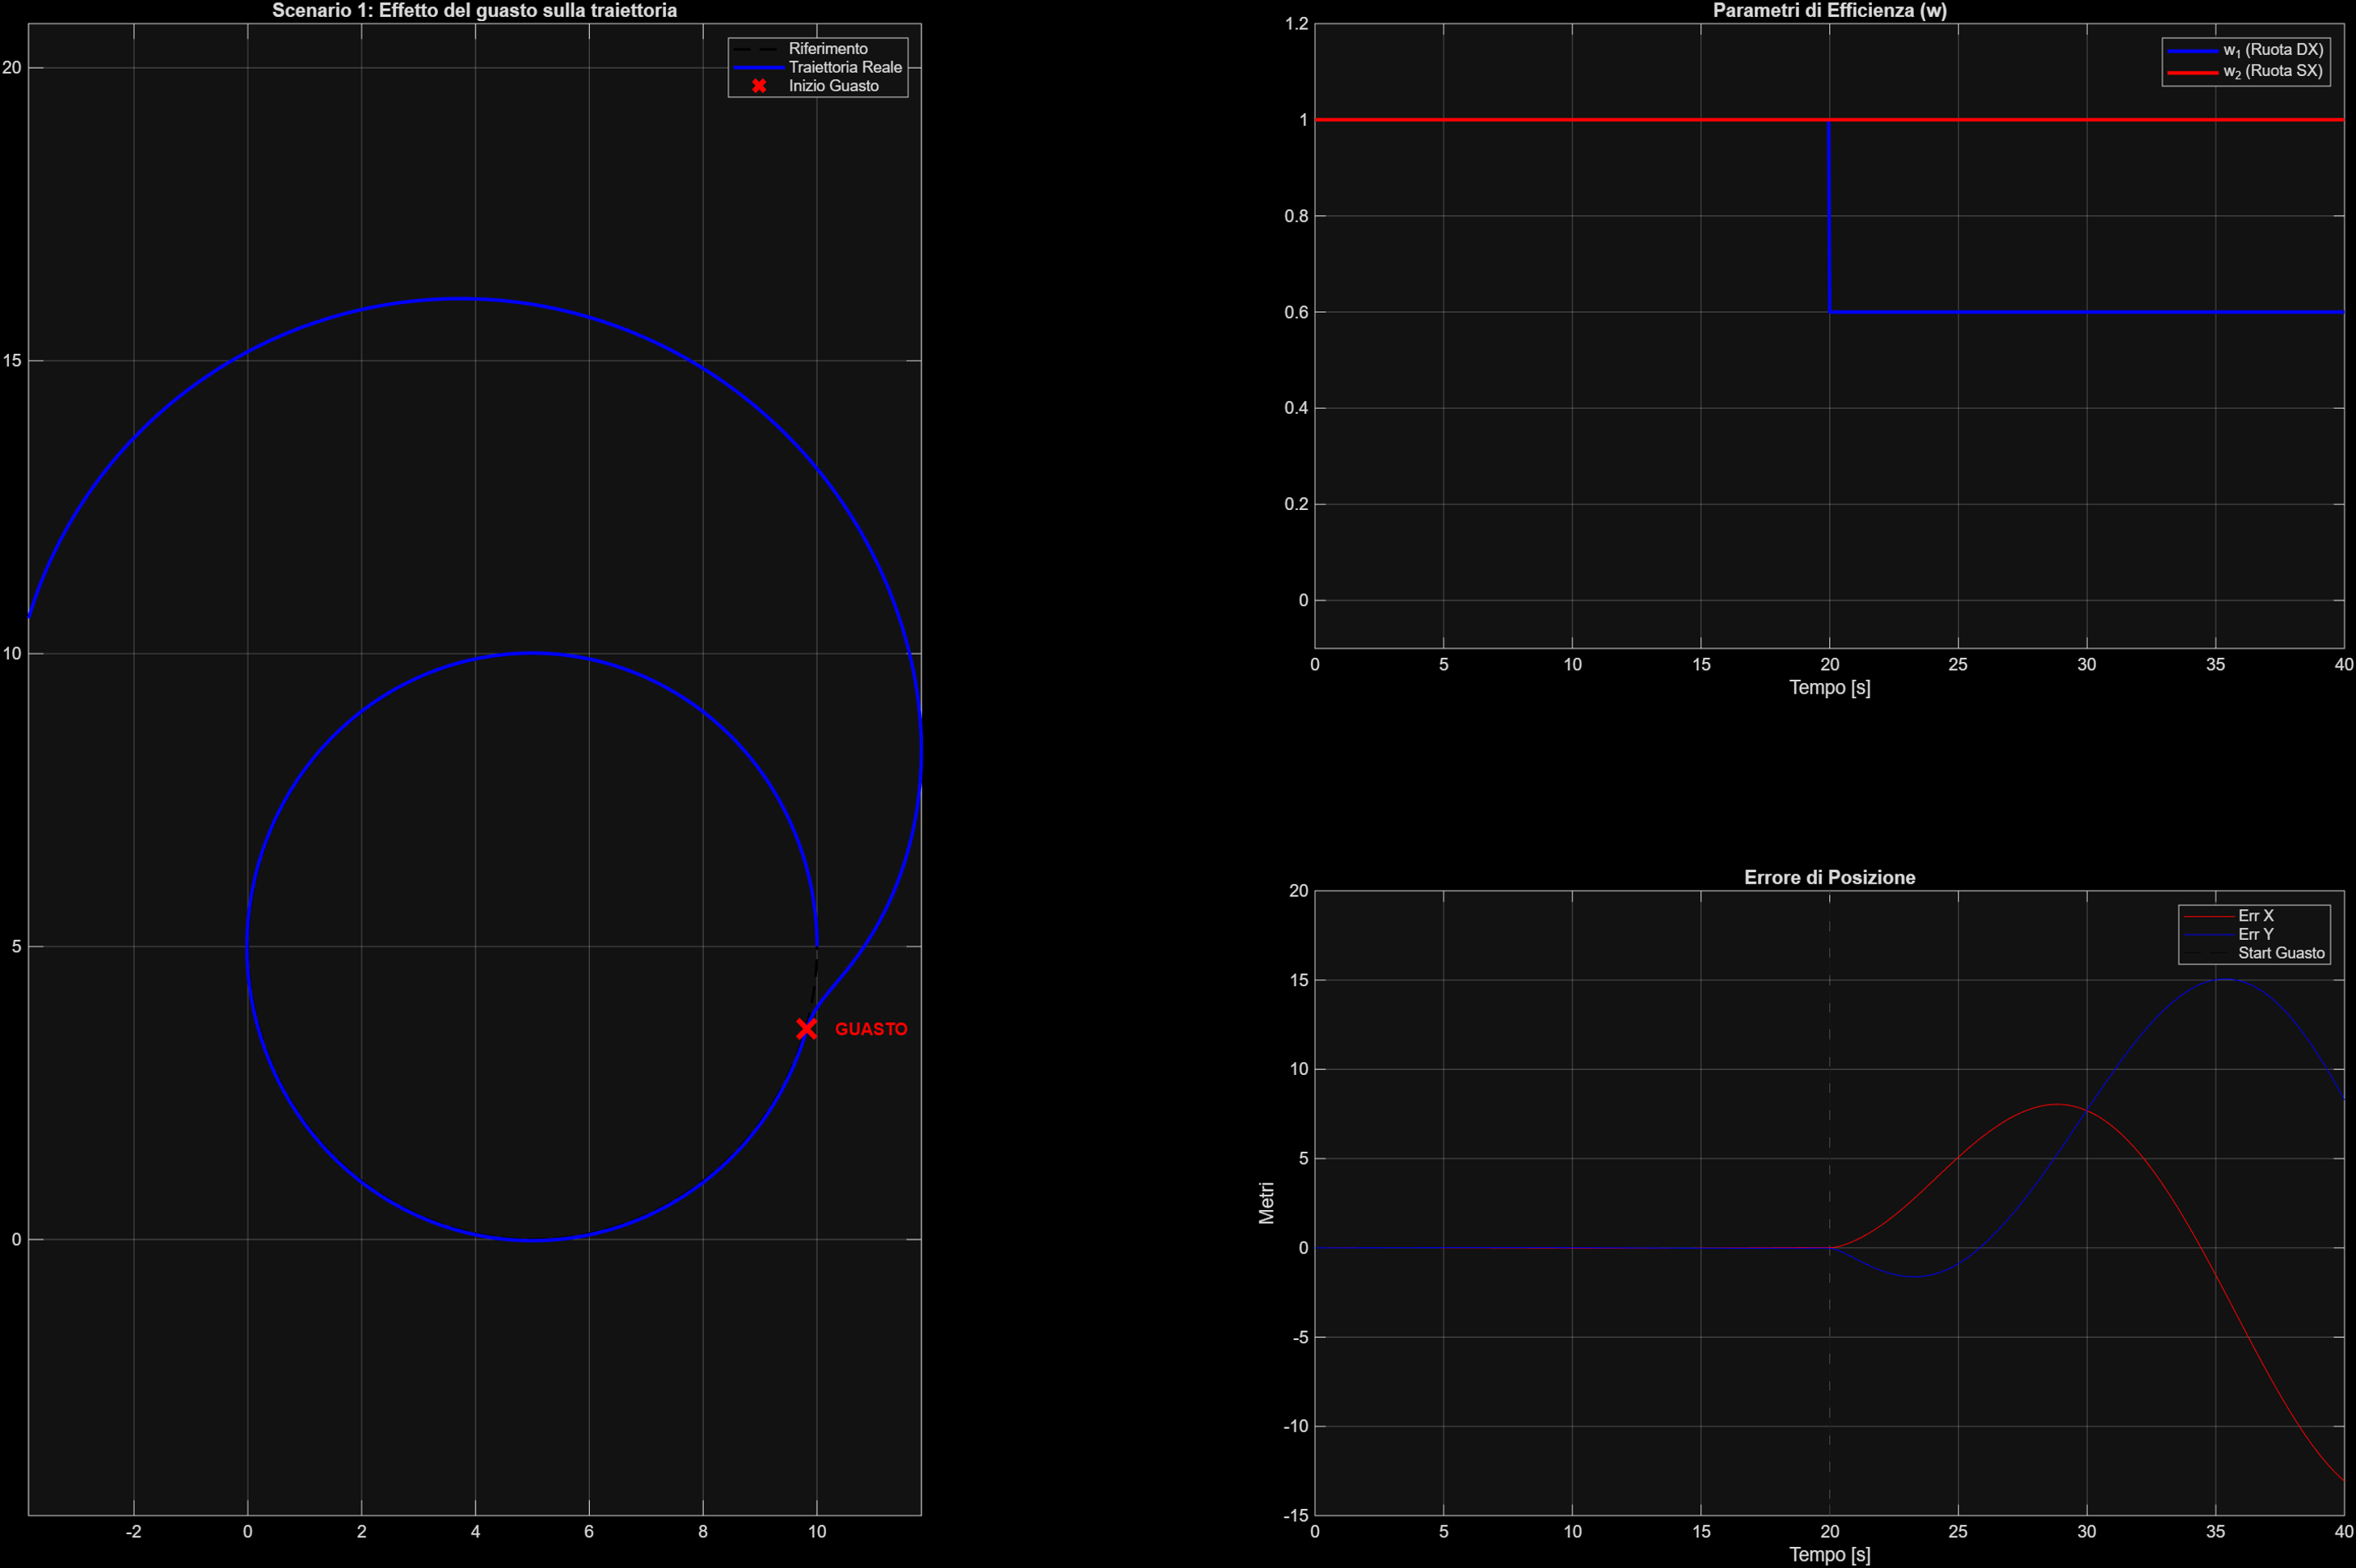
\includegraphics[width=1.0\textwidth]{chapter11/images/PuntoN3.png}
    \caption{Simulazione dello Scenario 1 (FD1): Effetto del guasto \( w_1=0.6 \) introdotto a \( t=20 \) s sulla traiettoria circolare.}
    \label{fig:punto3_results}
\end{figure}

\section{Conclusioni Punto 3}
La simulazione dimostra che i guasti agli attuatori degradano significativamente le prestazioni del sistema di controllo nominale. In particolare, un guasto asimmetrico (come il rallentamento di una sola ruota) introduce una perturbazione sulla dinamica rotazionale che porta il robot fuori traiettoria. Questo risultato evidenzia la necessità critica di un sistema di diagnosi (FDI) e di un controllo tollerante ai guasti (FTC), oggetto dei capitoli successivi.